
\documentclass[11pt,a4paper]{article}
\usepackage[T1]{fontenc}
\usepackage[utf8]{inputenc}
\usepackage{lmodern}
\usepackage{amsmath,amssymb}
\usepackage{graphicx}
\usepackage{booktabs}
\usepackage{array}
\usepackage{geometry}
\usepackage{setspace}
\usepackage{float}
\usepackage{caption}
\usepackage{siunitx}
\usepackage{xurl}
\usepackage[hidelinks]{hyperref}
\geometry{a4paper, margin=1in}
\setstretch{1.08}
\captionsetup{font=small,labelfont=bf}
\title{Claim-Bounded Diagnostics for Dark-Component-like SPARC Rotation-Curve Residuals:\\
Residual-Regime Mapping, Comparator Audits, and Null-Control Checks}
\author{Keiji Yoshimura\\Independent Researcher}
\date{May 2026\\\vspace{0.5em}\small GitHub repository: \url{https://github.com/yokken0907/dark-component-residual-response-audit}}
\begin{document}
\maketitle

\begin{abstract}
This manuscript presents a claim-bounded diagnostic audit of dark-component-like residual structure in SPARC galaxy rotation-curve data \cite{lelli2016}. The study is framed as a residual-regime mapping exercise, not as a physical dark-matter taxonomy, dark-matter exclusion claim, $\Lambda$CDM replacement, MOND/RAR falsification \cite{milgrom1983,mcgaugh2016}, NFW-halo falsification \cite{nfw1997}, Bullet-Cluster explanation, particle-identification inference, or Hubble-tension solution. Its narrower purpose is to ask whether residuals that are often described as dark-component-like can be organized into multiple diagnostic regimes using the previously developed SN-RRF parent result \cite{yoshimura2026snrrf}, NFW-like and RAR-like comparators, nuisance/pathology pass-through classes, proxy-association audits, and destructive/constructive null controls.

Across 143 eligible SPARC galaxies, the reported DCRRA protocol constructs a seven-zone residual-regime map. The final map contains 54 response-family-dominant galaxies, 23 response-family with NFW-competitive galaxies, 6 halo-comparator-dominant galaxies, 16 mixed three-way competitive galaxies, 30 nuisance-sensitive galaxies, 12 pathology/archive galaxies, and 2 unresolved triangular cases. The response-family-associated zones contain 77 galaxies, while pathology or nuisance pass-through classes contain 42 galaxies. DCRRA6 null controls reject destructive shuffled-label/proxy nulls in 4/4 tests and obtain nontrivial proxy-only reconstruction signals, with accuracy 0.314685 and balanced accuracy 0.328735. DCRRA8 locks the synthesis with 9/9 guards passed.

The safe conclusion is limited: within this diagnostic protocol and eligible SPARC subset, dark-component-like rotation-curve residuals are not treated as a single homogeneous category. They are represented as a claim-bounded residual-regime map containing response-family-like, halo-comparator-like, mixed, nuisance-sensitive, pathology/archive, and unresolved zones. This is a taxonomy for organizing residual behavior and validation priorities, not a causal physical classification and not a replacement for full dark-sector, modified-gravity, baryonic-feedback, lensing, cluster, or cosmological analyses.
\end{abstract}


\section*{Reader guidance and claim boundary}
This revised version is written to make the evidential status of the DCRRA package explicit before the technical construction begins. The manuscript should be read under the following boundaries.
\begin{itemize}
\item \textbf{Allowed interpretation.} The manuscript describes a claim-bounded diagnostic map of SPARC rotation-curve residual regimes under the reported DCRRA protocol.
\item \textbf{Not claimed.} The manuscript does not establish dark-matter exclusion, $\Lambda$CDM replacement, MOND/RAR falsification, NFW-halo falsification, Bullet-Cluster explanation, particle identity, Hubble-tension solution, or SN-RRF as a physical dark-matter substitute.
\item \textbf{Evidence status.} The reported zone counts, proxy associations, and null-control outcomes are treated as protocol-level diagnostic evidence in the eligible SPARC subset, not as independent observational validation of a physical dark-sector model.
\item \textbf{Role of comparators.} NFW-like, RAR-like, and SN-RRF-family-like models are used as diagnostic comparators. They are not exhaustive representatives of the full physical theory space.
\item \textbf{Next validation need.} Stronger claims require independent reproduction, alternative comparator sets, treatment of baryonic systematics, lensing and cluster-level checks, and expert evaluation against current galaxy-dynamics and cosmological pipelines.
\end{itemize}

\section{Scope and claim boundary}
DCRRA is built as a claim-bounded diagnostic taxonomy/audit of galaxy-scale residual behavior in the SPARC rotation-curve context \cite{lelli2016}. Its central purpose is to separate residual regimes, not to infer the physical identity or non-existence of dark matter. The following claims are explicitly outside the scope of this manuscript:
\begin{itemize}
\item dark-matter exclusion;
\item $\Lambda$CDM replacement;
\item MOND/RAR falsification;
\item NFW-halo falsification;
\item Bullet-Cluster explanation;
\item dark-matter particle identity;
\item Hubble-tension solution;
\item SN-RRF as a physical substitute for dark matter.
\end{itemize}
The allowed claim is narrower: dark-component-like SPARC rotation-curve residuals can be audited as multiple diagnostic residual regimes rather than as a single homogeneous category.

\section{Parent result and diagnostic motivation}
The parent result is the Scale-Normalized Residual Response Family (SN-RRF), developed from earlier A10/TVC-RRF fixed-kernel diagnostics \cite{yoshimura2026snrrf}. In the parent audit, the fixed exponent $n=3.258993$ was not retained as a unique universal law. Instead, the residual response was reformulated as a scale-normalized monotone-saturating family. The DCRRA project imports this parent result only as a diagnostic residual-response framework. It does not import it as a dark-matter substitute, physical TVC mechanism, unique fixed-exponent law, or cosmological replacement model.

For a dimensionless radius $s = r/R_{\rm last}$, a representative saturating kernel can be written as
\begin{equation}
K_n(x) = \frac{x^n}{1+x^n},\quad x = \frac{s}{s_c},
\end{equation}
where $s_c=r_c/R_{\rm last}$ is a scale-normalized response radius and $n$ is a response-shape parameter. DCRRA uses such quantities as diagnostic descriptors, not as microscopic physical laws.

\section{Pipeline summary}
The DCRRA pipeline proceeded through the following claim-bounded stages.
\begin{enumerate}
\item DCRRA0 locked the diagnostic-only scope and claim boundary.
\item DCRRA1 imported the SN-RRF parent result only as a diagnostic parent result.
\item DCRRA2 created a preliminary dark-component residual taxonomy.
\item DCRRA3 reclassified the SPARC population and audited stability relative to DCRRA2.
\item DCRRA4 performed a triangular NFW/RAR/SN-RRF comparator audit.
\item DCRRA5 tested environment/morphology/fit-proxy associations.
\item DCRRA6 performed destructive and constructive null controls.
\item DCRRA7 converted the preceding results into a residual-regime map.
\item DCRRA8 locked the claim-bounded synthesis and authorized the manuscript/repository package.
\end{enumerate}
No stage converts the residual map into a physical dark-matter taxonomy.

\section{Triangular comparator and proxy audits}
DCRRA4 compared NFW-like \cite{nfw1997}, RAR-like \cite{mcgaugh2016}, and SN-RRF-family-like \cite{yoshimura2026snrrf} diagnostic interpretations without treating the comparison as a cosmological model-selection claim. The audit separated the population into response-family, NFW-related, RAR-related/competitive, mixed, nuisance-sensitive, pathology/archive, and unresolved regimes.

DCRRA5 then tested whether the triangular residual-regime labels showed systematic association with proxy variables. Eight proxy binnings succeeded. Six proxies reached permutation $p\leq 0.05$, and all eight reached Cramer's $V \geq 0.25$. The strongest proxy association was the number of rotation-curve points. Significant associations also appeared for outer baryon-fraction proxy, gas-fraction proxy, best $n$, response radius $r_c/R_{\rm last}$, and response amplitude $A/v_{\rm outer}^2$. These are diagnostic associations only; they are not causal physical classifications.

\section{Destructive and constructive null controls}
DCRRA6 tested whether the DCRRA4 triangular classes were merely arbitrary labels. Destructive shuffled-label and shuffled-proxy nulls were rejected in 4/4 tests at $p\leq 0.05$. A proxy-only nearest-centroid constructive control recovered nontrivial class information, with accuracy 0.314685 and balanced accuracy 0.328735. Passing these controls supports proxy-coherent diagnostic structure, but it does not identify physical dark-matter categories.

\section{Residual-regime map}
DCRRA7 produced the final residual-regime map. The map contains seven zones and passes 8/8 guards. DCRRA8 then locks the synthesis with 9/9 guards passed. The zone counts are shown in Table~\ref{tab:zones} and Figure~\ref{fig:zonecounts}.

\begin{table}[H]
\centering
\caption{DCRRA residual-map zone counts for the 143-galaxy population.}
\label{tab:zones}
\small
\begin{tabular}{lrr}
\toprule
Residual-map zone & Count & Fraction \\
\midrule
RESPONSE\_FAMILY\_DOMINANT\_ZONE & 54 & 37.76\% \\
NUISANCE\_SENSITIVE\_ZONE & 30 & 20.98\% \\
RESPONSE\_FAMILY\_WITH\_NFW\_COMPETITIVE\_ZONE & 23 & 16.08\% \\
MIXED\_THREE\_WAY\_COMPETITIVE\_ZONE & 16 & 11.19\% \\
PATHOLOGY\_ARCHIVE\_ZONE & 12 & 8.39\% \\
HALO\_COMPARATOR\_DOMINANT\_ZONE & 6 & 4.20\% \\
UNRESOLVED\_TRIANGULAR\_ZONE & 2 & 1.40\% \\
\bottomrule
\end{tabular}
\end{table}

\begin{figure}[H]
\centering
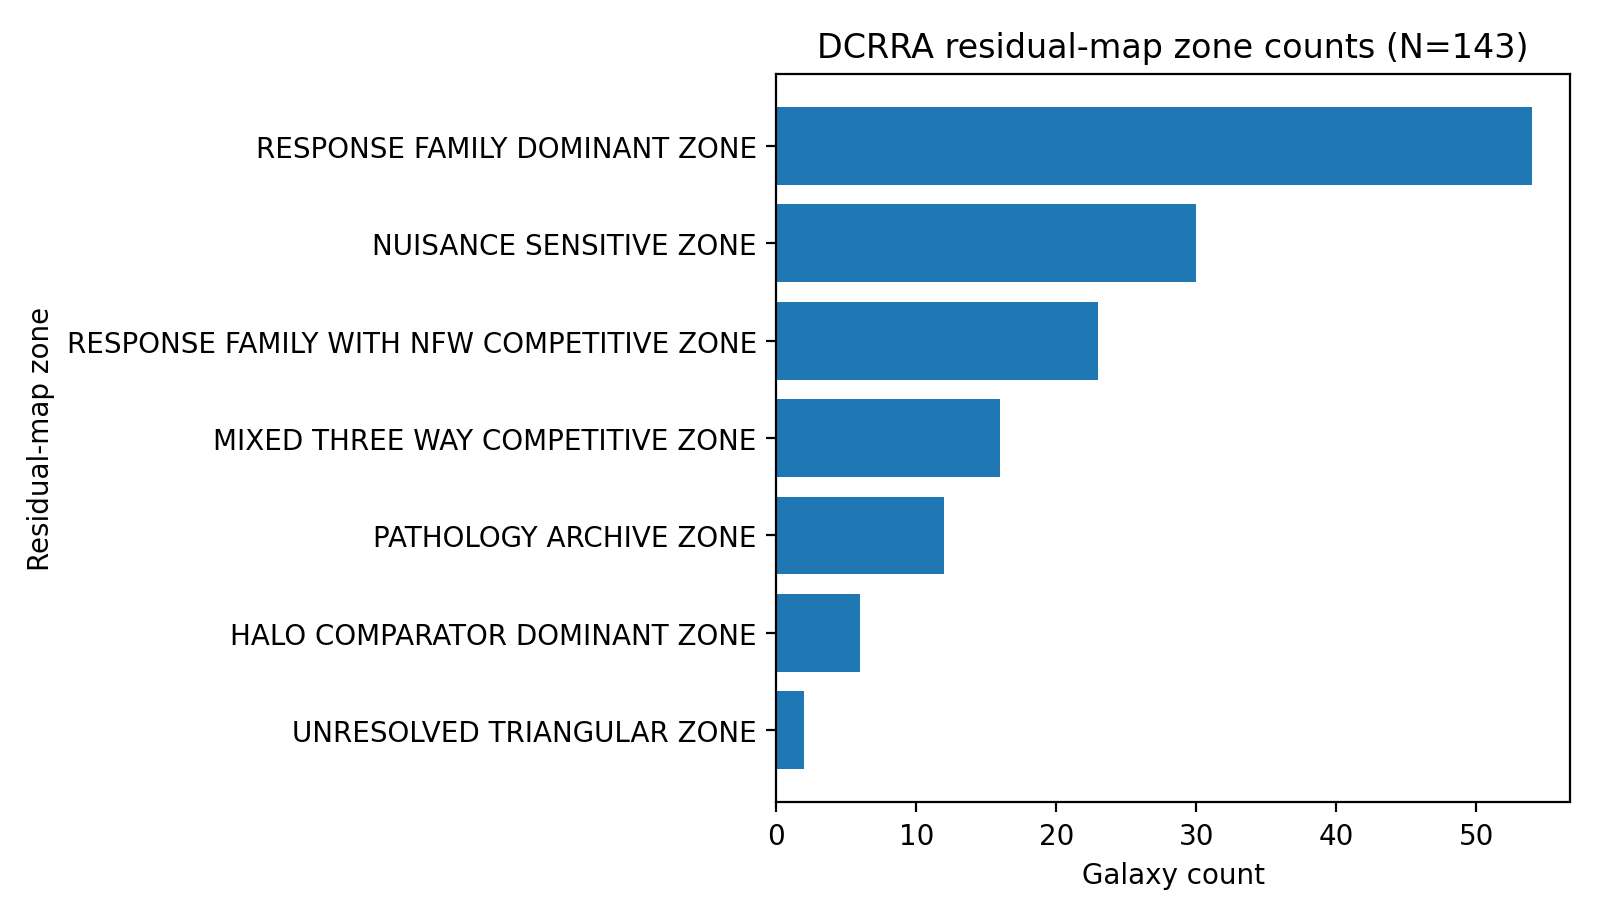
\includegraphics[width=0.94\linewidth]{../figures/dcrra_zone_counts.png}
\caption{Residual-map zone counts. The largest zone remains below a single-zone monopoly threshold, preserving a multi-regime interpretation.}
\label{fig:zonecounts}
\end{figure}

\section{Zone-level medians}
Table~\ref{tab:medians} summarizes key medians by zone. The response-family-dominant zone has median best $n=2.25$, median $r_c/R_{\rm last}=0.3335$, median $A/v_{\rm outer}^2=0.7805$, and strongly negative median diagnostic margins against both NFW-like and RAR-like comparators. The halo-comparator-dominant zone is small, with 6 galaxies, and has positive median family-minus-NFW margin, preserving an NFW-related diagnostic regime. Pathology/archive cases retain extreme or boundary-like descriptors and are not promoted into physical categories.

\begin{table}[H]
\centering
\caption{Selected residual-map zone medians. Negative $\Delta$AIC values indicate lower AIC \cite{akaike1974} for the SN-RRF-family diagnostic comparator relative to the named comparator.}
\label{tab:medians}
\scriptsize
\begin{tabular}{lrrrrrr}
\toprule
Zone & Count & best $n$ & $r_c/R_{\rm last}$ & $A/v_{\rm outer}^2$ & $\Delta$AIC fam-NFW & $\Delta$AIC fam-RAR \\
\midrule
Halo comp. dom. & 6 & 3 & 0.365 & 0.675 & 18.18 & -78.12 \\
Mixed 3-way & 16 & 2.5 & 0.365 & 0.724 & -2.49 & -2.41 \\
Nuisance sens. & 30 & 1.62 & 0.275 & 0.759 & -10.47 & -42.03 \\
Pathology/archive & 12 & 12 & 0.943 & 2.198 & -8.25 & -108.07 \\
Response dom. & 54 & 2.25 & 0.334 & 0.780 & -38.42 & -78.46 \\
Response + NFW comp. & 23 & 2.5 & 0.189 & 0.679 & -3.61 & -27.48 \\
Unresolved & 2 & 3.25 & 0.521 & 0.799 & -17.31 & -6.25 \\
\bottomrule
\end{tabular}
\end{table}

\begin{figure}[H]
\centering
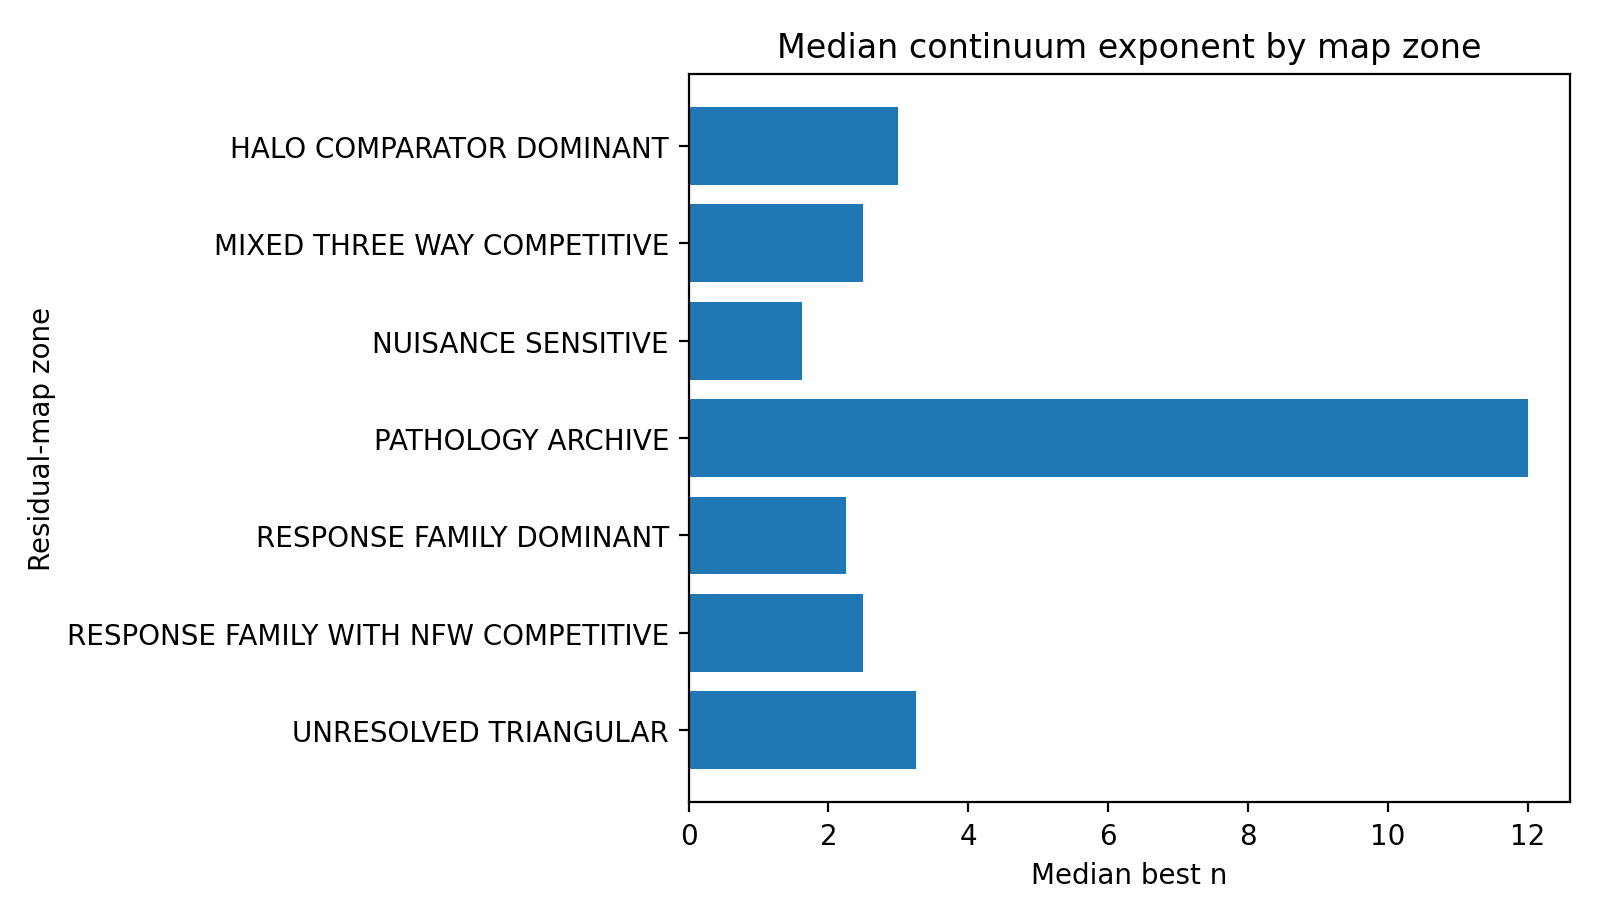
\includegraphics[width=0.94\linewidth]{../figures/dcrra_zone_median_best_n.png}
\caption{Median continuum exponent by residual-map zone. The spread reinforces the family-level interpretation rather than a universal fixed exponent.}
\label{fig:bestn}
\end{figure}

\section{Synthesis}
The central DCRRA result is a residual-regime map rather than a physical dark-matter taxonomy. The tested SPARC residual population is not monolithic. It separates into response-family-like, halo-comparator-like, mixed, nuisance-sensitive, pathology/archive, and unresolved regimes under the DCRRA protocol.

The most compact safe manuscript-level claim is:
\begin{quote}
Dark-component-like galaxy rotation-curve residuals can be audited as multiple diagnostic residual regimes rather than as a single homogeneous category. In the tested SPARC population, a response-family-associated zone is prominent, but NFW-comparator, mixed, nuisance-sensitive, pathology/archive, and unresolved regimes remain explicitly preserved.
\end{quote}

This language is intentionally weaker than a discovery claim about the nature of dark matter and stronger than a purely descriptive table: it says that a structured, null-controlled diagnostic decomposition exists under the tested protocol.

\section{Limitations}
Several limitations are essential. First, the map is based on SPARC rotation-curve residuals and does not include direct lensing constraints, galaxy clusters, CMB structure formation, or direct-detection experiments. Second, the NFW-like and RAR-like components are comparators in a diagnostic audit, not exhaustive representatives of their full theoretical model classes. Third, proxy associations are not causal explanations. Fourth, nuisance-sensitive and pathology/archive zones are preserved rather than repaired or reinterpreted. Finally, the pipeline does not determine whether dark matter exists, what its particle identity is, or whether modified gravity or baryonic feedback provides a better physical explanation.

\section{Conclusion}
DCRRA0-DCRRA8 support a claim-bounded diagnostic map of dark-component-like SPARC galaxy rotation-curve residuals. In 143 eligible galaxies, the final seven-zone map contains 77 response-family-associated cases, 6 halo-comparator-dominant cases, 16 mixed cases, 42 pathology/nuisance pass-through cases, and 2 unresolved cases. The maximum single-zone fraction is 0.377622, avoiding collapse into a single homogeneous category. DCRRA6 null controls support proxy-coherent structure, and DCRRA8 locks the synthesis with 9/9 guards passed.

The result should be used as a diagnostic residual-regime map. It should not be described as dark-matter exclusion, $\Lambda$CDM replacement, MOND/RAR falsification, NFW falsification, Bullet-Cluster explanation, particle-identification inference, Hubble-tension solution, or a physical dark-matter substitute.



\section*{Repository and reproducibility availability}
\sloppy
The repository package associated with this manuscript is available at \url{https://github.com/yokken0907/dark-component-residual-response-audit}. Versioned repository releases may be archived on Zenodo as repository-archive records for reproducibility, provenance, and citation of the public release package. Such Zenodo identifiers refer to archived repository releases, not to separately peer-reviewed article DOIs, and they do not broaden the claim boundary beyond the diagnostic residual-regime map stated in the manuscript. The previous repository archive record for the original framing was \href{https://doi.org/10.5281/zenodo.20233908}{10.5281/zenodo.20233908}. A future Zenodo DOI generated for a revised GitHub release should be interpreted in the same repository-archive sense.
\fussy

\section*{Acknowledgments}
Large language models, including OpenAI ChatGPT, were used as research-assistance tools for theory structuring, verification-protocol organization, code drafting, numerical-audit workflow design, and manuscript editing support. The author remains responsible for the final scientific claims, claim boundaries, interpretation, and manuscript content.

\begin{thebibliography}{99}
\bibitem{akaike1974} H. Akaike, A new look at the statistical model identification, IEEE Transactions on Automatic Control 19(6), 716--723 (1974). DOI: 10.1109/TAC.1974.1100705.
\bibitem{lelli2016} F. Lelli, S. S. McGaugh, and J. M. Schombert, SPARC: Mass Models for 175 Disk Galaxies with Spitzer Photometry and Accurate Rotation Curves, The Astronomical Journal 152, 157 (2016). DOI: 10.3847/0004-6256/152/6/157.
\bibitem{mcgaugh2016} S. S. McGaugh, F. Lelli, and J. M. Schombert, Radial Acceleration Relation in Rotationally Supported Galaxies, Physical Review Letters 117, 201101 (2016). DOI: 10.1103/PhysRevLett.117.201101.
\bibitem{milgrom1983} M. Milgrom, A modification of the Newtonian dynamics as a possible alternative to the hidden mass hypothesis, The Astrophysical Journal 270, 365--370 (1983). DOI: 10.1086/161130.
\bibitem{nfw1997} J. F. Navarro, C. S. Frenk, and S. D. M. White, A Universal Density Profile from Hierarchical Clustering, The Astrophysical Journal 490, 493--508 (1997). DOI: 10.1086/304888.
\bibitem{yoshimura2026snrrf} K. Yoshimura, Scale-Normalized Residual Response Family for SPARC Galaxy Rotation-Curve Residuals: From A10/TVC-RRF Fixed-Kernel Diagnostics to Dimensionless Manifold and Kernel-Family Synthesis, independent manuscript and repository package (2026). DOI: 10.5281/zenodo.20224479.

\bibitem{yoshimura2026dcrra} K. Yoshimura, Claim-Bounded Diagnostics for Dark-Component-like SPARC Rotation-Curve Residuals: Residual-Regime Mapping, Comparator Audits, and Null-Control Checks, independent manuscript and repository package (2026). Repository archive history: \href{https://doi.org/10.5281/zenodo.20233908}{10.5281/zenodo.20233908}. GitHub repository: \url{https://github.com/yokken0907/dark-component-residual-response-audit}.

\end{thebibliography}

\end{document}
